% Working draft for the Madrid LEZ manuscript.
\documentclass[runningheads]{llncs}

\usepackage[T1]{fontenc}
\usepackage{graphicx}
\usepackage{url}
\usepackage{amsmath}
\usepackage{amssymb}
\usepackage{booktabs}
\usepackage{cite}
\usepackage{hyperref}
\usepackage{textcomp}
\usepackage{float}
\usepackage{placeins}

\begin{document}

\title{Robust Counterfactual Forecasting for Testing Post-Policy Air-Quality Deviations in Madrid}
\titlerunning{Testing Post-Policy Deviations in Madrid}

\author{Gilberto J. Brito\inst{1}\orcidID{0009-0000-9011-4009} \and
Manuel Curado\inst{1}\orcidID{0000-0003-2307-1760} \and
Marc Semper\inst{1}\orcidID{0000-0001-5974-8062} \and
Jose F. Vicent\inst{1}}

\authorrunning{G. J. Brito et al.}

\institute{Department of Computer Science and Artificial Intelligence, University of Alicante, Alicante, Spain\\
\email{gjb3@alu.ua.es, manuel.curado@ua.es, marc.semper@ua.es, jvicent@ua.es}}

\maketitle

\begin{abstract}
This article tests whether post-policy air-quality observations in selected Madrid districts remain below a pre-policy predictive baseline under compact robustness checks. The data combine hourly pollution, district traffic intensity, and meteorological information for Salamanca, Tetuan, and Villa de Vallecas. Models are trained on 2021 pre-policy observations and then used to forecast the pollutant levels expected under continuation of the pre-policy regime during 2022--2023. The main comparison covers Ridge, LightGBM, and a stacked multivariate LSTM with temporal windows of 6 and 24 hours, together with naive seasonal baselines, feature ablations, sensitivity to IQR-based outlier filtering, fixed-horizon placebo boundaries, a rolling-origin backtest, and a direct-evaluation sensitivity. LightGBM with a 6-hour window provides the best main-split validation accuracy, reaching a mean MAE of 17.90 and outperforming the strongest seasonal-naive benchmark at 20.52. Under that specification, post-policy observations remain lower than the no-change forecast on average (mean PIP 70.18\%, mean residual 4.32), with 95\% day-block bootstrap intervals of [69.32, 71.15] for PIP and [3.71, 5.01] for the mean residual. In a 60-day comparison, the January 2022 boundary yields larger positive gaps than late-2021 placebo cuts, although that placebo contrast is supportive rather than dispositive. Rolling-origin validation keeps LightGBM as the preferred model family, although 6- and 12-hour windows are close. Removing meteorological variables weakens the signal more than removing district traffic intensity, so the findings should be read as post-policy deviations after adjustment for weather and available urban covariates rather than as identification of a traffic mechanism. The evidence therefore supports a local predictive signal compatible with lower observed post-policy concentrations relative to the no-change forecast, while stopping well short of strong causal claims or city-wide generalization.

\keywords{Low-emission zones \and Counterfactual forecasting \and Air quality \and Time series \and Robustness analysis}
\end{abstract}

\section{Introduction}\label{sec:introduction}

Urban air pollution remains a persistent public-health and environmental problem, especially in dense metropolitan areas where traffic emissions, atmospheric conditions, and land-use patterns interact over time \cite{Dominski2021}. Low-emission zones (LEZs), pedestrianization, and related mobility restrictions have therefore become common policy tools for reducing exposure to traffic-related pollutants. Their evaluation is methodologically demanding because air quality changes are shaped not only by regulation but also by weather, seasonality, traffic redistribution, and local urban form.

This study approaches that problem through predictive counterfactuals. The core idea is to estimate forecasting models using only the pre-policy regime and then compare their expected pollution levels with the realized observations after the policy boundary. Such a design is attractive because it can exploit rich multivariate time series, but it is only persuasive when the substantive conclusion survives reasonable choices about model class, temporal context, input information, and placebo boundaries. A positive result observed under a single architecture or a single preprocessing recipe is difficult to defend as policy evidence.

The article therefore asks a narrower but more defensible question: do post-policy pollution levels in the selected Madrid districts remain systematically below the no-change forecast under a compact but robust forecasting design? The emphasis is on stability rather than on rhetorical force. The goal is not to claim definitive causal identification, but to test whether the post-policy deviation persists when the counterfactual is confronted with stronger baselines, placebo cuts, and lightweight sensitivity checks.

The manuscript makes four concrete contributions. First, it compares Ridge, LightGBM, and LSTM against strong naive benchmarks. Second, it studies temporal context through 6- and 24-hour main windows plus a supplementary 12-hour rolling-origin sensitivity. Third, it complements PIP with mean and median post-policy residuals, bootstrap intervals, and late-2021 placebo boundaries. Fourth, it uses feature ablations, a direct-evaluation sensitivity, and explicit local framing for the three-district panel rather than suggesting city-wide generalization.

\section{Related Work}\label{sec:related}

The literature most relevant to this manuscript sits at the intersection of two strands that do not always talk to each other. One strand evaluates LEZs or related mobility restrictions as public policy and emphasizes treatment timing, comparison groups, and the interpretation of post-policy changes in regulated pollutants. Recent examples report measurable improvements in traffic-related air quality while also stressing trade-offs, spillovers, and heterogeneous local effects \cite{PRIETORODRIGUEZ2022237,SARMIENTO2023105014}. This strand is useful for motivating the policy question, but its identification logic often differs from the forecasting-based design used here.

The second strand focuses on air-quality forecasting itself. Here the dominant concern is predictive accuracy rather than policy evaluation. Prior work has explored machine-learning and deep-learning models for pollutant prediction under different feature sets, including meteorology-only inputs, traffic-related covariates, and mixed-source data \cite{SAMAD2023119987,Rahman2024}. These studies show that multivariate forecasting can capture meaningful pollutant dynamics, but they usually stop at prediction performance and do not translate the forecasts into a policy counterfactual.

This paper uses forecasting to test post-policy deviations rather than as an end in itself. Models are trained only on the pre-policy regime and then used to estimate what pollution levels would have looked like in the absence of the post-policy shift. In that sense, the forecasting model plays the role of a counterfactual generator. The approach is closer in spirit to event-based designs that compare observed outcomes with an expected baseline \cite{Guo2021}, but it remains prediction-driven rather than fully econometric. The gap addressed here is the relative scarcity of compact, robustness-oriented studies that combine both perspectives without letting the conclusion rest on a single preferred specification.

\section{Study Area and Data}\label{sec:data}

The empirical setting consists of three Madrid districts with distinct urban profiles and mobility patterns: Salamanca, Tetuan, and Villa de Vallecas. The analysis uses hourly records from 2021--2023, with 2021 treated as the pre-policy period and 2022--2023 treated as post-policy observations after the first circulation restrictions considered here came into force on 1 January 2022 under the 2021 amendment to Madrid's Sustainable Mobility Ordinance \cite{OrdenanzaMovilidadMadrid2021}. This district-level design keeps the policy question local, which is appropriate because both traffic intensity and pollutant behavior can vary sharply across urban environments.

The data architecture combines official datasets from the Madrid Open Data Portal \cite{MadridOpenDataPortal}: hourly air-quality records, hourly meteorological records, historical traffic measurements, and traffic-point location files. Air-quality series provide the target pollutants. Meteorological covariates account for atmospheric conditions that can alter pollutant concentration independently of policy changes. Traffic measurements and district-level traffic intensity act as proxies for local mobility conditions that may covary with post-policy deviations, without by themselves identifying a mobility mechanism. In the final panel, one air-quality station is retained per district, district traffic is taken from the hourly aggregation produced by the project notebooks, and meteorological variables are rebuilt as hourly city-wide averages to avoid the sparsity left by the initial merge.

The purpose of this section is to define what enters the model and why, rather than to reproduce a long narrative about district demographics. Table~\ref{tab:variables} summarizes the variables and their role in the forecasting design. One practical limitation should be made explicit: PM$_{2.5}$ is unavailable for the retained Villa de Vallecas station in the final panel, so that pollutant is not reported for that district in the result tables.

\begin{table}[htbp]
\centering
\caption{Variables used in the counterfactual forecasting design}
\label{tab:variables}
\begin{tabular}{@{}ll@{}}
\toprule
\multicolumn{2}{@{}l}{\textbf{Input features}} \\
\cmidrule(r){1-2}
Variable & Description \\
\midrule
Calendar encoding & Cyclic hour, weekday, month, and day-of-year features \\
Historical pollutant values & Autoregressive lags used by Ridge and LightGBM \\
Wind speed & Wind intensity \\
Wind direction & Prevailing wind direction \\
Temperature & Ambient temperature \\
Relative humidity & Humidity level \\
Barometric pressure & Atmospheric pressure \\
Solar radiation & Solar-radiation intensity \\
Precipitation & Rainfall indicator or amount \\
District traffic intensity & District-level traffic aggregation \\
\midrule
\multicolumn{2}{@{}l}{\textbf{Target pollutants}} \\
\cmidrule(r){1-2}
Variable & Description \\
\midrule
NO & Nitric oxide concentration \\
NO$_2$ & Nitrogen dioxide concentration \\
NO$_x$ & Nitrogen oxides concentration \\
PM$_{10}$ & Particulate matter below 10\textmu m \\
PM$_{2.5}$ & Particulate matter below 2.5\textmu m \\
\bottomrule
\end{tabular}
\end{table}

The exact feature bundle varies slightly by model family. Ridge and LightGBM use pollutant-specific historical lags together with district traffic, meteorology, and cyclic calendar features, whereas the stacked multivariate LSTM uses windows of exogenous and calendar information and predicts the pollutant vector jointly. The substantive question is not whether these data can support a single apparently strong forecast, but whether the sign and magnitude of the post-policy gaps remain stable when model family, temporal context, and feature availability are deliberately perturbed.

\section{Counterfactual Forecasting Framework}\label{sec:framework}

\subsection{Predictive Counterfactual Formulation}

The forecasting task is defined over district-level time series. For Ridge and LightGBM, a separate model is estimated for each pollutant $p$ using autoregressive windows that combine the recent history of that pollutant with district traffic, meteorology, and cyclic calendar features. If $x_t$ denotes the exogenous and calendar features at time $t$ and $y_t^{(p)}$ the concentration of pollutant $p$, the pollutant-specific forecast has the generic form
\[
\hat{y}_t^{(p)} = f_{\theta}^{(p)}(y_{t-w}^{(p)}, \ldots, y_{t-1}^{(p)}, x_{t-w}, \ldots, x_{t-1}).
\]

The stacked LSTM is instead estimated as a multivariate sequence model. It uses windows of exogenous and calendar inputs and predicts the pollutant vector jointly:
\[
\hat{\mathbf{y}}_t = g_{\theta}(x_{t-w}, \ldots, x_{t-1}),
\]
where $\hat{\mathbf{y}}_t$ contains the five pollutant forecasts at time $t$. At post-policy times, the counterfactual predictions represent the pollution levels expected under continuation of the pre-policy regime, whereas the realized observations reflect the post-policy setting.

The interpretation is intentionally modest. Positive gaps of the form $\hat{y}_t - y_t > 0$ are treated as evidence consistent with lower observed post-policy concentrations relative to the no-change forecast. They are not treated as proof of strong causal identification, because the model-based counterfactual remains sensitive to predictive misspecification and to the information encoded in the pre-policy period.

The estimand also matters for how predictions are generated after the boundary. For the autoregressive Ridge and LightGBM models, a recursive rollout is required if the forecast is meant to represent continuation of the pre-policy regime. Feeding observed post-policy pollutant lags back into the model would update the autoregressive state with treated outcomes and would therefore answer a different question. A direct one-step evaluation based on observed post-policy lags is still informative as a symmetry check for predictive ranking, but not as the primary no-change counterfactual.

\subsection{Preprocessing}

The preprocessing pipeline consists of district assignment for sensors, temporal alignment of air-quality, meteorological, and traffic records, hourly reindexing over 2021--2023, interpolation of missing exogenous values, and feature scaling where required by the model family. An IQR-based outlier treatment is retained as a clipping rule applied to pre-policy ranges so that the hourly sequence remains continuous for forecasting. Rather than treating that rule as unquestioned preprocessing, the empirical design evaluates its removal as a sensitivity case.

To keep the paper concise, generic textbook descriptions of forecasting metrics are omitted. What matters here is the sequence of design choices that can plausibly change the sign or magnitude of the post-policy comparison.

\subsection{Temporal Windows}

Temporal dependence is tested with two explicit windows in the main design: $w=6$ and $w=24$. These choices represent short-term and day-scale context, respectively, and are long enough to test whether additional temporal memory changes the inferred post-policy signal while keeping the comparison compact and interpretable.

Using only two windows in the core tables is a deliberate design choice. The objective is not an exhaustive hyperparameter search, but a targeted robustness check. If the sign of the policy-consistent effect changes materially between $w=6$ and $w=24$, then the substantive interpretation becomes more fragile. If it remains directionally stable, the result is easier to defend. A supplementary rolling-origin sensitivity later introduces $w=12$ only to verify that the preferred short-range window is not an artifact of the main split.

\subsection{Compared Models}

The extended manuscript compares three model families chosen to cover distinct inductive biases without expanding the paper beyond its editorial scope.

\paragraph{\textbf{Ridge}}
Ridge regression is the linear benchmark. It provides a transparent baseline and helps determine whether the post-policy signal already appears under a restricted linear specification.

\paragraph{\textbf{LightGBM}}
LightGBM represents a strong non-linear machine-learning baseline for tabular data. In this context it captures feature interactions and non-linearities without requiring a heavier architectural commitment. The model is fitted on flattened historical windows, which makes it directly comparable to the linear baseline while preserving the same temporal context.

\paragraph{\textbf{LSTM}}
The LSTM model provides the sequential deep-learning alternative \cite{10.1162/neco.1997.9.8.1735}. In the implemented comparison, it is specified as a stacked five-layer multivariate network with dropout after each LSTM block and joint prediction of the five pollutants. This design preserves a recognizably sequential architecture while keeping the model comparison manageable.

The model set is intentionally limited to these three families. Adding graph neural networks or transformers would increase implementation cost and discussion burden without clearly improving the interpretability of a compact policy-oriented comparison. The available data benefit more from controlled robustness than from architectural proliferation.

\subsection{Effect Summaries}

Post-policy behavior is summarized first through the positive impact percentage (PIP), defined as the share of post-policy observations for which the counterfactual prediction exceeds the realized value:
\[
\mathrm{PIP} = \left( \frac{1}{N} \sum_{i=1}^{N} \mathbf{1}(\hat{y}_i > y_i) \right) \times 100.
\]

PIP is supplemented with two signed residual summaries:
\[
\mathrm{MR} = \frac{1}{N} \sum_{i=1}^{N} (\hat{y}_i - y_i),
\qquad
\mathrm{MdR} = \mathrm{median}_{i=1,\ldots,N} (\hat{y}_i - y_i).
\]
Here $\mathrm{MR}$ is the mean residual and $\mathrm{MdR}$ is the median residual over the post-policy period. Positive values indicate that observed pollution is lower than the no-change forecast, whereas negative values indicate the opposite. Using all three summaries gives a more informative picture than PIP alone because it separates directional consistency from effect magnitude and reduces dependence on outliers.

\section{Experimental Design}\label{sec:design}

The empirical protocol begins by defining 1 January 2022 as the main policy boundary. This leaves the full year 2021 for model estimation and the years 2022--2023 for post-policy evaluation. Models are fitted only on pre-policy data. Within that period, the first 70\% of 2021 is used for training and the last 30\% for validation.

Model selection is performed in the pre-policy regime. The primary metric for selecting the best specification is mean absolute error (MAE), reported by pollutant and then summarized compactly across pollutants and districts. The main text focuses on MAE and treats post-policy metrics separately. The principal specification is chosen exclusively on this pre-declared main split. The rolling-origin exercise is a robustness check for family-level stability and short-window stability, not a second model-selection stage. For Ridge and LightGBM, validation and post-policy prediction are recursive because the estimand is a no-change continuation of the pre-policy autoregressive path. The multivariate LSTM is evaluated over observed exogenous windows because it predicts the pollutants jointly in a direct fashion. A separate direct-evaluation sensitivity is reported later to compare model families under a more homogeneous one-step setup, but it is not used as the main counterfactual because it conditions on observed post-policy pollutant lags.

The study evaluates the following model-and-data configurations:
\begin{itemize}
\item full feature set with Ridge, LightGBM, and LSTM;
\item two naive benchmarks: one-hour persistence and same-hour previous-day seasonal naive forecasting;
\item temporal windows of 6 and 24 steps;
\item a supplementary rolling-origin sensitivity with windows of 6, 12, and 24 steps for the preferred model family;
\item an ablation without traffic variables;
\item an ablation without meteorological variables;
\item a sensitivity run without IQR-based outlier removal;
\item a fixed-horizon placebo comparison using late-2021 boundaries;
\item a direct one-step evaluation sensitivity for comparing model families under a more homogeneous prediction scheme.
\end{itemize}

This is intentionally a minimal robustness design. It is broad enough to test whether the post-policy conclusion depends on one particular source of information or one specific preprocessing choice, but narrow enough to keep the interpretation readable. More aggressive ablation grids would increase the number of tables and the discussion burden without proportionate gain.

Once the best pre-policy specification is identified, post-policy forecasts are generated for each pollutant and district. The evaluation then aggregates the realized post-policy gaps using PIP, mean residual, and median residual. Uncertainty for those aggregate summaries is approximated with a 500-repetition block bootstrap that resamples whole days, which preserves short-range autocorrelation better than pointwise resampling. Temporal specificity is checked with 60-day placebos at 1 October 2021 and 1 November 2021, compared with the first 60 days after 1 January 2022 under the same preferred model. District-level reporting is essential because the substantive claim is local rather than city-wide, and heterogeneous responses across Salamanca, Tetuan, and Villa de Vallecas are plausible on substantive grounds.

More extensive resampling or hyperparameter exploration is left for future work. The present design prioritizes a compact comparison and a small set of robustness checks that can be defended within a short article. Even after the added placebos and rolling-origin checks, the contribution remains a local predictive assessment rather than a city-wide or strongly causal estimate.

\section{Results}\label{sec:results}

Table~\ref{tab:model_selection} summarizes the pre-policy model-selection stage together with the naive benchmarks. The best average validation performance is obtained by LightGBM with a 6-step window, which reaches a mean MAE of 17.90 across the valid district-pollutant combinations. Among the learned models, LightGBM with a 24-step window is the second-best configuration at 20.60. The strongest naive comparator is the same-hour previous-day forecast at 20.52, while one-hour persistence is much weaker at 31.74. The stacked multivariate LSTM remains clearly weaker than LightGBM on average, and Ridge produces the largest post-policy gaps but also by far the worst pre-policy MAE. In other words, the most optimistic post-policy summaries are not attached to the most credible predictive baseline.

\begin{table}[htbp]
\centering
\caption{Pre-policy model-selection summary with learned models and naive baselines; post-policy PIP is shown only as a secondary reference}
\label{tab:model_selection}
\begin{tabular}{@{}lrrrr@{}}
\toprule
Model & Window & Mean MAE & Median MAE & Mean post PIP (\%) \\
\midrule
LightGBM & 6  & 17.90 & 13.36 & 70.18 \\
Seasonal naive & 24 & 20.52 & 16.88 & 68.85 \\
LightGBM & 24 & 20.60 & 15.58 & 73.24 \\
LSTM     & 6  & 24.02 & 14.32 & 18.97 \\
LSTM     & 24 & 24.12 & 14.52 & 17.88 \\
Persistence & 1  & 31.74 & 24.70 & 91.72 \\
Ridge    & 6  & 36.16 & 32.82 & 84.13 \\
Ridge    & 24 & 36.43 & 32.82 & 92.35 \\
\bottomrule
\end{tabular}
\end{table}

The naive baselines sharpen two points. First, the preferred LightGBM $w=6$ model improves on the strongest naive comparator by 2.62 MAE points, so the selected specification is not merely reproducing a simple daily seasonal heuristic. Second, the persistence forecast attains the largest mean post-policy PIP despite poor pre-policy fit, reinforcing why PIP should not be interpreted without a credible predictive baseline.

A supplementary rolling-origin check within 2021 keeps LightGBM as the preferred family and shows that the exact short-range window is not unique. Over three 30-day folds, LightGBM attains mean MAE values of 13.28 for $w=6$, 13.04 for $w=12$, and 13.62 for $w=24$, all better than the seasonal-naive benchmark at 14.74. The manuscript nevertheless retains $w=6$ as the principal specification because model selection is fixed exclusively by the pre-declared main split, where $w=6$ clearly outperforms the supplementary $w=12$ sensitivity (17.90 vs.\ 21.02 mean MAE). The rolling-origin exercise is used only to assess family-level stability and short-window stability, not to reopen model selection after seeing the main result.

The preferred specification is therefore the full-feature LightGBM model with window $w=6$. Table~\ref{tab:ablation_summary} summarizes the post-policy behavior of that specification under the main ablations. The full model yields a mean PIP of 70.18\%, a mean residual of 4.32, and a median residual of 4.93. Removing traffic leaves the aggregate signal almost unchanged, whereas removing meteorological variables lowers the mean PIP to 65.29\% and roughly halves the mean residual. The no-IQR run preserves the average PIP but worsens pre-policy MAE and increases the mean residual, which suggests that the outlier treatment affects magnitude more than direction. The no-traffic ablation attains a slightly smaller MAE (17.46 vs.\ 17.90), but the ablations are used as diagnostics rather than as a second model-selection stage, and the full model is retained because it preserves a substantively relevant mobility covariate even when its incremental predictive contribution is limited in this panel.

\begin{table}[htbp]
\centering
\caption{Post-policy summary for the preferred LightGBM $w=6$ specification and its minimal ablations}
\label{tab:ablation_summary}
\begin{tabular}{@{}lrrrr@{}}
\toprule
Variant & Mean MAE & Mean PIP (\%) & Mean residual & Median residual \\
\midrule
Full model & 17.90 & 70.18 & 4.32 & 4.93 \\
No traffic & 17.46 & 70.08 & 4.55 & 4.79 \\
No weather & 18.56 & 65.29 & 2.04 & 4.39 \\
No IQR     & 19.81 & 70.44 & 6.16 & 3.83 \\
\bottomrule
\end{tabular}
\end{table}

Uncertainty in the preferred post-policy summaries is modest at the aggregate level. A day-block bootstrap with 500 repetitions yields a 95\% interval of [69.32, 71.15] for mean PIP, [3.71, 5.01] for the mean residual, and [4.43, 5.34] for the median residual. These intervals remain on the positive side of zero for the residual-based summaries, so the aggregate signal is not driven by a small set of isolated hours.

Figures~\ref{fig:placebo} and \ref{fig:tradeoff} provide complementary diagnostics on temporal specificity and the fit-gap trade-off. Figure~\ref{fig:placebo} shows a fixed 60-day placebo exercise for the preferred LightGBM $w=6$ model. The January 2022 boundary yields larger positive gaps than the late-2021 placebo cuts: mean residual 8.96 and mean PIP 75.12\% against 6.77 and 73.54\% for October 2021, and 4.98 and 71.84\% for November 2021. The placebo contrast is supportive but not dispositive. Figure~\ref{fig:tradeoff} shows the trade-off between pre-policy fit and post-policy gap. The most spectacular gaps belong to weak baselines such as Ridge and persistence, whereas LightGBM offers the strongest predictive credibility with a still-positive aggregate deviation.

A direct one-step sensitivity with observed histories provides a more homogeneous comparison across model families. Under that sensitivity, LightGBM still has the best predictive ranking by MAE (9.28 for $w=6$ against 12.33 for Ridge and 24.02 for LSTM), but the mean post residual is -1.40. The reason is substantive rather than contradictory: once treated post-policy lags are inserted into the forecast window, the model is no longer estimating continuation of the untreated pre-policy regime. It is answering a different one-step prediction question. The direct sensitivity therefore strengthens the model-ranking argument, but not the no-change counterfactual itself.

At the district-pollutant level, the pattern remains positive in many cells but not uniformly so. Figure~\ref{fig:heatmap} shows the mean residuals for the preferred specification. PM$_{10}$ is the strongest and most consistent positive signal, especially in Villa de Vallecas, where the mean residual reaches 18.42 and PIP rises to 87.56\%. By contrast, NO is the least stable pollutant: its mean residual is slightly negative in all three districts even though PIP remains above 65\%, which illustrates why PIP alone is not sufficient to characterize the post-policy behavior. PM$_{2.5}$ is not reported for Villa de Vallecas because the retained station does not provide valid measurements for that pollutant in the final panel.

The traffic ablation needs a similarly local reading. Its aggregate effect is small, but not identically zero. Removing the district traffic proxy changes the Tetuan NO$_2$ mean residual by 2.74 and its PIP by 3.24 points. The available traffic variable is therefore not inert, but it is too coarse to support a strong mechanism claim.

\begin{figure}[htbp]
\centering
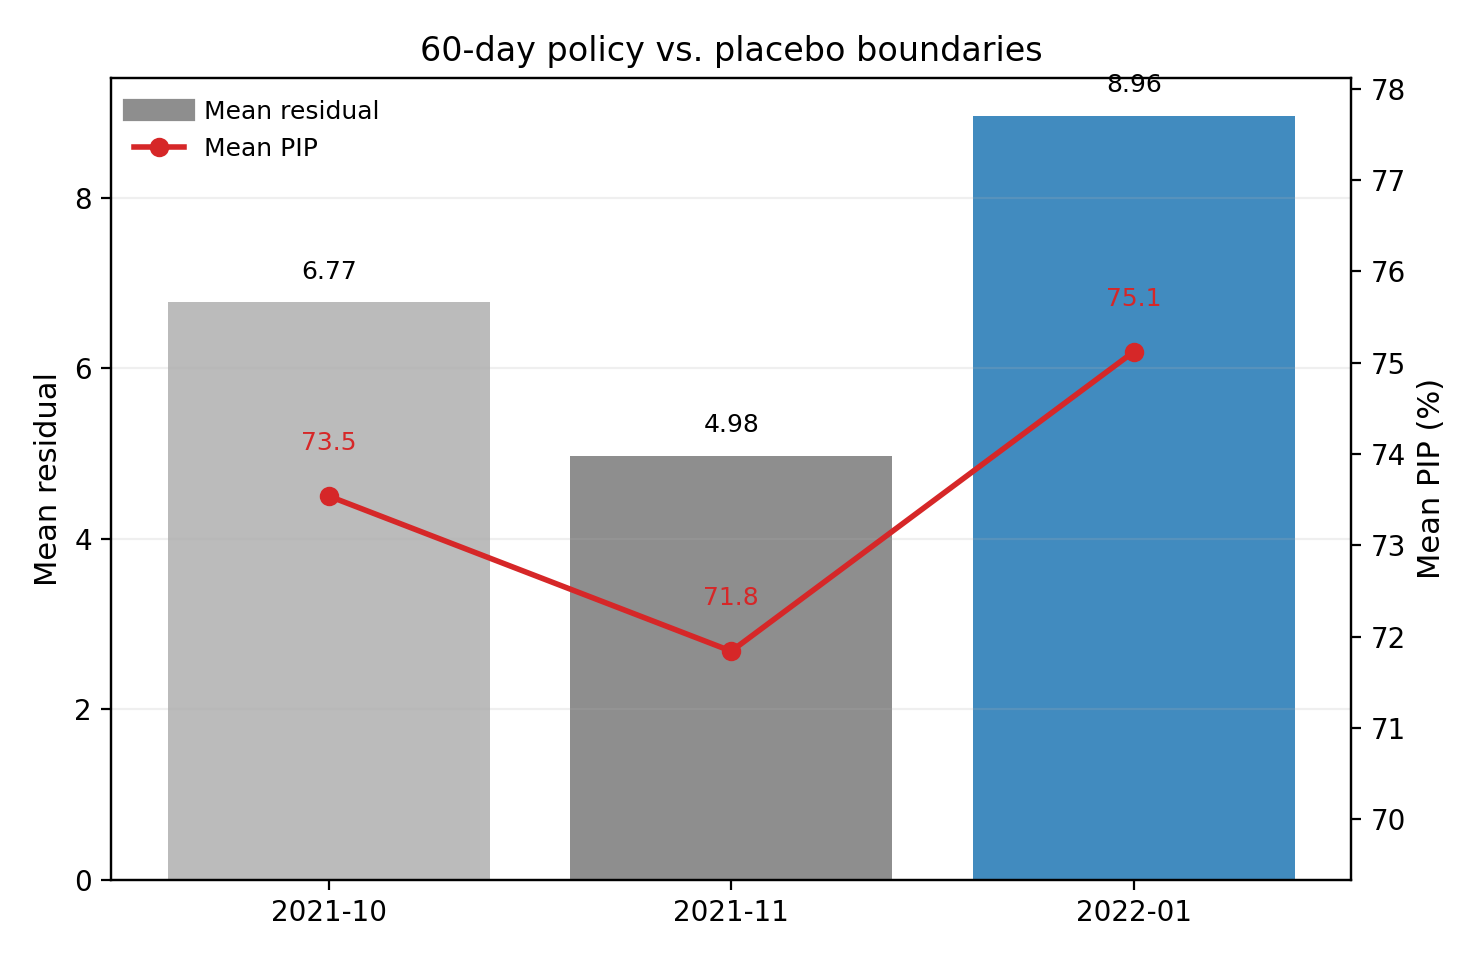
\includegraphics[width=.68\linewidth]{figures/placebo_boundary_comparison.png}
\caption{Fixed 60-day comparison between late-2021 placebo boundaries and the January 2022 policy boundary for the preferred LightGBM model with $w=6$.}
\label{fig:placebo}
\smallskip
\noindent\textit{Alt text: Bar chart comparing mean residual and mean PIP over the 60 days following October 2021, November 2021, and January 2022 boundaries. The January 2022 bars are the highest in both metrics.}
\end{figure}

\begin{figure}[htbp]
\centering
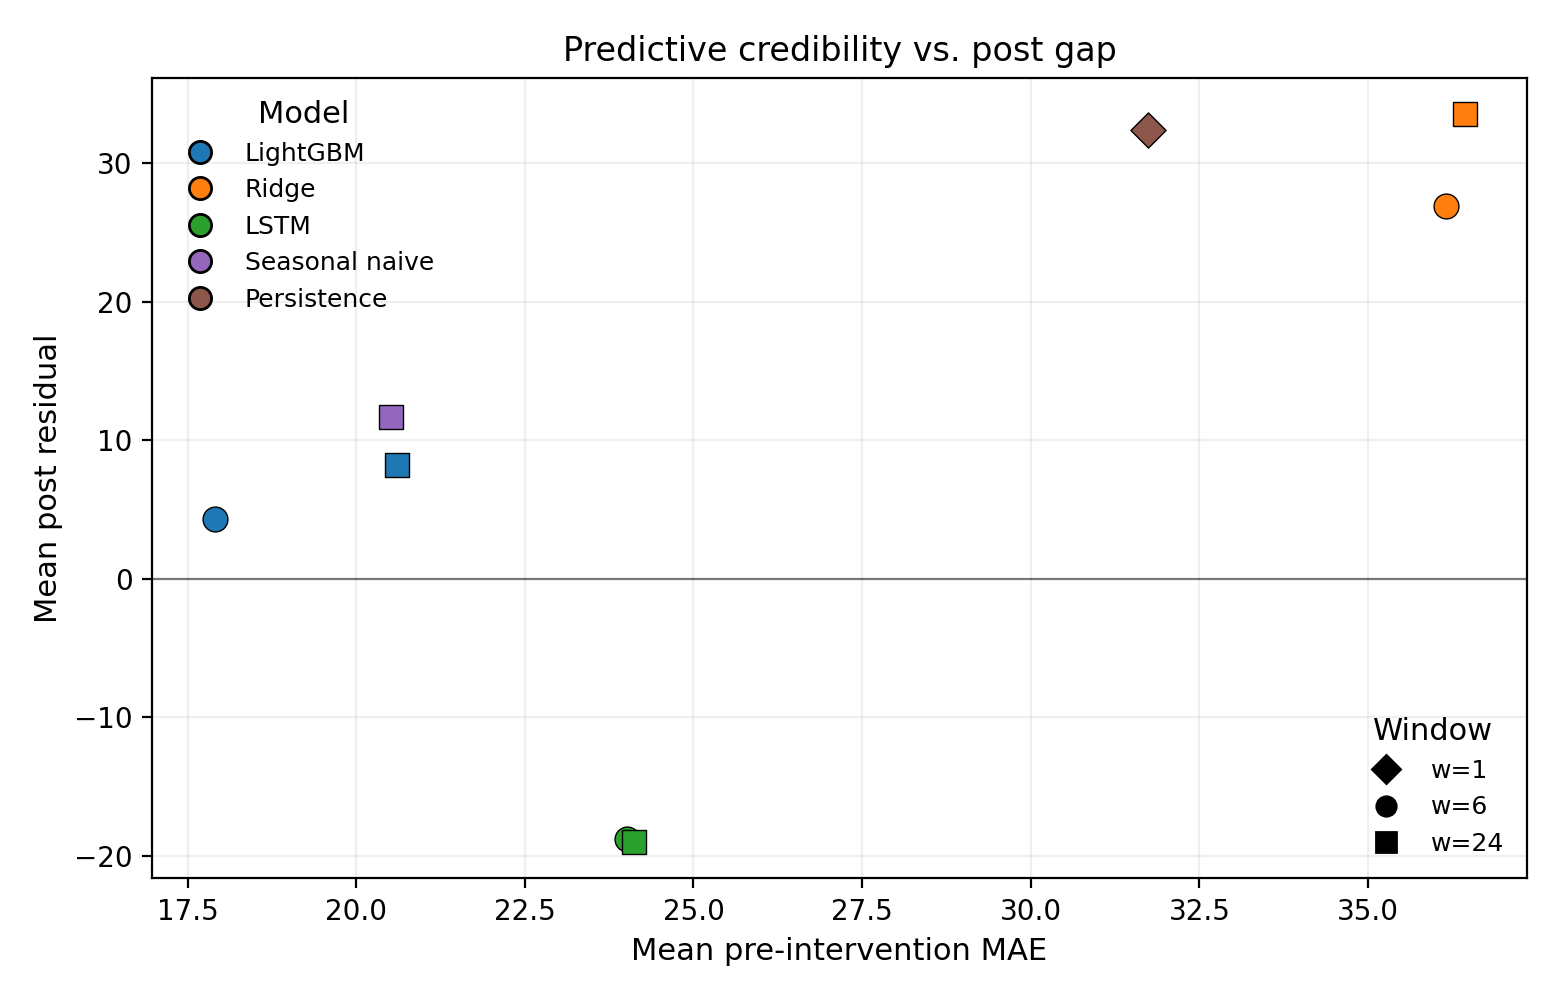
\includegraphics[width=.68\linewidth]{figures/credibility_tradeoff.png}
\caption{Relation between pre-policy MAE and mean post residual across learned models and naive baselines.}
\label{fig:tradeoff}
\smallskip
\noindent\textit{Alt text: Scatter plot of pre-policy MAE versus mean post residual, with colors for model family and marker shapes for window choice. LightGBM clusters in the lower-error region, while Ridge and persistence occupy higher-error regions with larger gaps.}
\end{figure}

\begin{figure}[htbp]
\centering
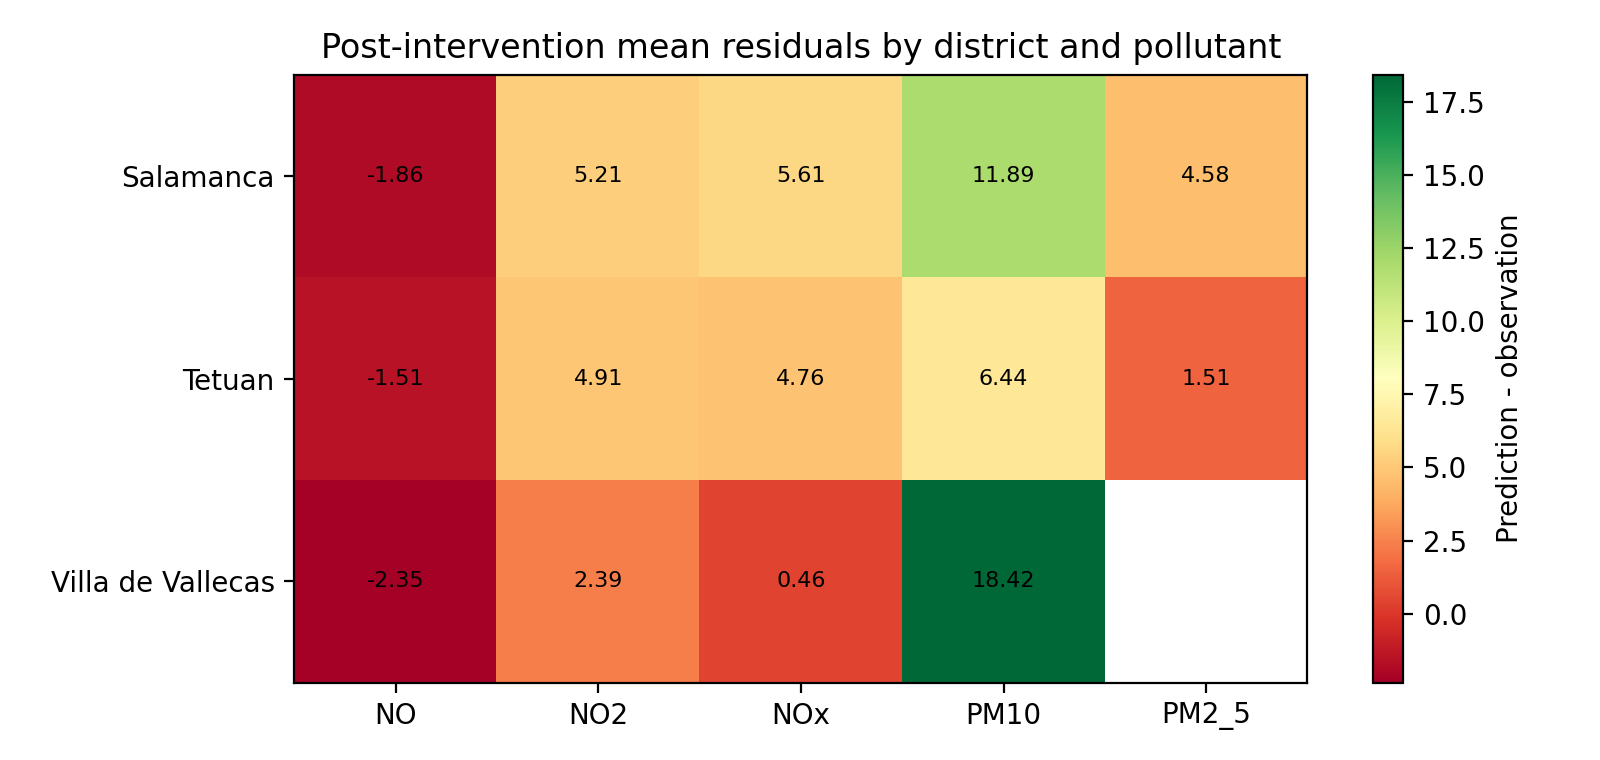
\includegraphics[width=.80\linewidth]{figures/best_full_variant_heatmap.png}
\caption{Post-policy mean residuals ($\hat{y} - y$) for the preferred full-feature LightGBM model with window $w=6$}
\label{fig:heatmap}
\smallskip
\noindent\textit{Alt text: Heatmap with districts on the vertical axis and pollutants on the horizontal axis. Most cells are positive, indicating observed pollution below the counterfactual forecast, with the strongest positive value for PM$_{10}$ in Villa de Vallecas and small negative NO residuals across the three districts.}
\end{figure}

\section{Robustness and Discussion}\label{sec:discussion}

The empirical results should be interpreted through robustness rather than rhetoric. LightGBM remains the most credible baseline, whereas Ridge achieves larger gaps only with much poorer fit and the stacked LSTM fails to preserve a convincing average post-policy signal. The rolling-origin check also keeps LightGBM preferred, although $w=6$ and $w=12$ are close enough that the exact short-range window should not be overinterpreted.

The added diagnostics strengthen but do not settle the case. The preferred model beats the naive baselines, retains positive bootstrap intervals, and its 60-day January 2022 boundary is stronger than the nearby October and November 2021 placebos. Yet the placebo cuts are not null. The placebo contrast is supportive but not dispositive, and the forecasting design attenuates temporal drift rather than eliminating it.

The traffic and evaluation sensitivities mainly clarify interpretation. Removing meteorology weakens the signal more than removing district traffic intensity, so the result should be read as a deviation after adjustment for weather and available urban covariates, not as identification of a traffic mechanism. The small MAE advantage of the no-traffic ablation is therefore diagnostic rather than dispositive: it shows limited incremental predictive contribution from the available district proxy, not that mobility information is substantively irrelevant. Likewise, a homogeneous direct one-step evaluation keeps LightGBM best by MAE but attenuates the gap once observed post-policy lags enter the window. That is exactly what should happen: the empirical question changes once treated lags replace the untreated autoregressive path. Recursive rollout therefore remains necessary for the no-change estimand.

The district narrative and the external-validity claim must therefore stay local. The strongest positive cell is PM$_{10}$ in Villa de Vallecas, whereas NO remains slightly negative in the three districts. This is evidence of local heterogeneity in the selected districts and retained stations, not proof of a city-wide causal effect.

\section{Conclusions}\label{sec:conclusions}

This study tests whether post-policy air-quality observations in a local three-district Madrid panel remain below a pre-policy predictive baseline under robustness checks. The central idea is simple: train forecasting models on the pre-policy regime and examine whether the observed post-policy path falls below the no-change forecast after broader model comparison, temporal sensitivity analysis, and placebo checks.

The practical value of the design lies in its discipline. The case study remains focused on three districts and on the combination of air-quality, district traffic intensity, and meteorological information, but the empirical logic is strengthened through Ridge, LightGBM, and LSTM comparisons, naive seasonal benchmarks, windows of 6 and 24 steps, a supplementary 12-step rolling-origin sensitivity, feature ablations, fixed-horizon placebos, and sensitivity to outlier filtering. The results select LightGBM with a 6-step window as the best main-split pre-policy specification by MAE, while the rolling-origin check keeps LightGBM as the preferred family even when the exact short window is not unique. The stacked multivariate LSTM remains weaker than LightGBM overall, which suggests that, in this setting, a strong tabular baseline is more reliable than a more expressive sequential alternative.

Under that preferred specification, the post-policy signal remains positive on average, with a mean PIP of 70.18\% and a positive mean residual of 4.32. The same model also outperforms persistence and seasonal-naive forecasting, its aggregate post-policy summaries remain positive under day-block bootstrap intervals, and its first 60 post-policy days are more favorable than the nearby late-2021 placebo boundaries. At the same time, the new comparison shows why stronger controls matter: Ridge can produce much larger apparent effects, but it does so with substantially worse pre-policy fit. The ablations also indicate that meteorological information matters more than district traffic intensity for preserving the signal in this dataset, while the IQR-based preprocessing mainly affects magnitude rather than direction.

The final claim should therefore remain cautious. The evidence supports a local post-policy deviation that is compatible with lower observed post-policy concentrations relative to the no-change forecast; it does not provide definitive proof of a causal effect, a traffic mechanism, or city-wide generalization. Nearby placebos are weaker than the January 2022 boundary, but they are not null, so some temporal drift remains. The placebo contrast is supportive but not dispositive. That narrower claim is scientifically stronger because it is anchored in explicit model comparison, visible placebo checks, genuine temporal sensitivity, and compact robustness checks rather than in a single favorable architecture.

The code used to generate the empirical results is available at \url{https://github.com/Semllo/Robust-Counterfactual-Forecasting}, together with instructions for retrieving the official Madrid Open Data sources named in Section~\ref{sec:data}.

\subsection*{Funding}
This research received no specific grant from any funding agency in the public, commercial, or not-for-profit sectors.


\bibliographystyle{splncs04}
\bibliography{bibliography}

\end{document}
